% !TeX spellcheck = pt_BR
%%%%%%%%%%%%%%%%%%%%%%%%%%%%%%%%%%%%%%%%%%%%%%%%%%%%%%%%%%%%%%%%%%%%%%%%%%%%%%%%%%%%%%%%%%%%%%%%
%                                                                                              %
%                             Definicao para a classe Artigo                                   %
%                                                                                              %
%%%%%%%%%%%%%%%%%%%%%%%%%%%%%%%%%%%%%%%%%%%%%%%%%%%%%%%%%%%%%%%%%%%%%%%%%%%%%%%%%%%%%%%%%%%%%%%%

\documentclass[portugues, brazil, a4paper,12pt]{article}
\bibliographystyle{plain}

%%%%%%%%%%%%%%%%%%%%%%%%%%%%%%%%%%%%%%%%%%%%%%%%%%%%%%%%%%%%%%%%%%%%%%%%%%%%%%%%%%%%%%%%%%%%%%%%
%                                                                                              %
%                       Pacotes a utilizar na compilacao do documento                          %
%                                                                                              %
%%%%%%%%%%%%%%%%%%%%%%%%%%%%%%%%%%%%%%%%%%%%%%%%%%%%%%%%%%%%%%%%%%%%%%%%%%%%%%%%%%%%%%%%%%%%%%%%

\usepackage[brazil]{babel}
\usepackage{graphicx}
\usepackage{geometry}
\usepackage[utf8]{inputenc}
\usepackage[T1]{fontenc}
\usepackage{algorithm}
\usepackage{color}
\usepackage{minted}
%\usepackage{algorithmic}
\usepackage[noend]{algpseudocode}
\usepackage{epstopdf}
\usepackage{hyperref}
\usepackage{todonotes}
\usepackage{amsmath}
\usepackage{verbatim}
\usepackage{gensymb}

\hypersetup{
    colorlinks,
    citecolor=black,
    filecolor=black,
    linkcolor=black,
    urlcolor=black
}



\makeatletter
\renewcommand{\paragraph}{\@startsection{paragraph}{4}{0ex}%
   {-3.25ex plus -1ex minus -0.2ex}%
   {1.5ex plus 0.2ex}%
   {\normalfont\normalsize\bfseries}}
\makeatother

\stepcounter{secnumdepth}
\stepcounter{tocdepth}

%%%%%%%%%%%%%%%%%%%%%%%%%%%%%%%%%%%%%%%%%%%%%%%%%%%%%%%%%%%%%%%%%%%%%%%%%%%%%%%%%%%%%%%%%%%%%%%%
%                                                                                              %
%                       Configuracao dos pacotes utilizados no doc.                            %
%                                                                                              %
%%%%%%%%%%%%%%%%%%%%%%%%%%%%%%%%%%%%%%%%%%%%%%%%%%%%%%%%%%%%%%%%%%%%%%%%%%%%%%%%%%%%%%%%%%%%%%%%

\geometry{a4paper,left=3cm,right=3cm,top=2.5cm,bottom=2.93cm}


%%%%%%%%%%%%%%%%%%%%%%%%%%%%%%%%%%%%%%%%%%%%%%%%%%%%%%%%%%%%%%%%%%%%%%%%%%%%%%%%%%%%%%%%%%%%%%%%
%                                                                                              %
%                             Capa do relatorio tecnico                                        %
%                                                                                              %
%%%%%%%%%%%%%%%%%%%%%%%%%%%%%%%%%%%%%%%%%%%%%%%%%%%%%%%%%%%%%%%%%%%%%%%%%%%%%%%%%%%%%%%%%%%%%%%%

\begin{document}

\begin{titlepage}

  \vfill

	\begin{figure}[H]
	\centering
		
\includegraphics[scale=0.15]{img/logo-ufop.jpg}
	\end{figure}

  \vfill

  \begin{center}
    \begin{Large}
      \textbf{UNIVERSIDADE FEDERAL DE OURO PRETO}
    \end{Large}
  \end{center}

  \begin{center}
    \begin{large}
      \textbf{Mestrado em Ciência da Computação} \\[1.4cm]
    \end{large}
  \end{center}

  \vfill

  \begin{center}
    \begin{large}
      \textbf{Especificação Sistêmica de Carro Robô Seguidor de Linha com Sistema Avançado Utilizando Controle Proporcional}
    \end{large}
  \end{center}

  \vfill

  \begin{center}
    \begin{large}
      Autor: \\
		Rodolfo Labiapari Mansur Guimarães - \url{rodolfolabiapari@decom.ufop.br}
    \end{large}
  \end{center}

	\vfill

  \begin{center}
    \begin{large}
      Professor: \\
      Ricardo Augusto Rabelo Oliveira - \url{rrabelo@gmail.com}
    \end{large}
  \end{center}

  \vfill

  \begin{center}
    \begin{large}
      Ouro Preto - MG \\
      \today \\
    \end{large}
  \end{center}

\clearpage
\tableofcontents
\end{titlepage}

%%%%%%%%%%%%%%%%%%%%%%%%%%%%%%%%%%%%%%%%%%%%%%%%%%%%%%%%%%%%%%%%%%%%%%%%%%%%%%%%%%%%%%%%%%%%%%%%
%                                                                                              %
%                               Introducao ao trabalho                                         %
%                                                                                              %
%%%%%%%%%%%%%%%%%%%%%%%%%%%%%%%%%%%%%%%%%%%%%%%%%%%%%%%%%%%%%%%%%%%%%%%%%%%%%%%%%%%%%%%%%%%%%%%%

\part{Especificação de Projeto Embarcado}


\section{Introdução}
	Esta Parte I consiste em uma especificação de um trabalho de sistema embarcado complexo a ser construído em uma Parte II.

	Atualmente é possível construir Carro Robô Seguidor de Linha utilizando poucos componentes, e com poucas linhas de programação, além da facilidade em encontrar em sites de venda de eletrônicos kits de sensores e atuadores de baixo custo prontos para serem acoplados à placa de prototipagem e assim, a construção de um carro seguidor.

	O desenvolvimento do sistema controlador também segue o mesmo princípio de facilitação de uso. Utilizando uma plataforma de prototipagem tal como Arduino, é possível escrever o controle de um carro seguidor com poucas linhas de instruções. Isso pode ser levado como um desafio até para crianças e adolescentes com criatividade e entusiasmo para desenvolver um sistema completo e funcional como incentivo à robótica.

	Na Seção \ref{sec:especificacao} será exibido a especificação deste trabalho e na Seção \ref{sec:rt} é feito toda a introdução teórica sobre o tema. Em Seção \ref{sec:elem-teo} é descrito com detalhes todos os elementos que serão utilizados para fazer este projeto ser concretizado, em \ref{sec:math} é feito uma exibição das definições matemáticas que o projeto levará em consideração para seu funcionamento e por fim, na Seção \ref{sec:arch} é descrito como será a arquitetura escolhida para comunicação e processamento das informações.


\section{Especificações} \label{sec:especificacao}

	Abaixo é escrito a especificação segundo Professor Rabelo Oliveira \href{mailto:rrabelo@gmail.com}{rrabelo@gmail.com}.
	\begin{verbatim}
		Neste trabalho, o robô será controlado por uma instância externa na Cloud, que
		ira efetuar a leitura dos dados transmitidos pelo robo via NodeMCU para
		retornar como feedback para os atuadores.
		O caminho executado/aprendido pelo robô deverá ser usado para controlar um
		segundo robô que não possui sensores. Considere o ponto de partida similar
		para ambos.
		A programação do segundo robo será enviada pela Cloud que contem os dados
		e algoritmo do primeiro robo.
		O trabalho consistirá em duas entregas
		Primeira Entrega - Especificação do projeto: devera conter de maneira
		detalhada as seguintes características:
		a- Referencial teórico
		b- Proposta dos sensores do primeiro robo
		c- Proposta dos atuadores dos robos, explicando como serão programados
		d- Alimentação do sistema, indicando como sera montada a parte da
		alimentação dos motores e do NodeMCU
		e- Modelo matemático considerando os dados dos sensores discretos.
		f- A SOLUÇÃO DA EQUAÇÃO DEVERA SER DISCRETA
		SOMENTE DE PRIMEIRA ORDEM
		g- Arquitetura para a execução do controle de primeira ordem nas nuvens
		e o envio dos dados pela internet, Indicar a solução de Cloud para uso (azure,
		amazon, watson, etc)
		Data entrega:08/02/2017
	\end{verbatim}


\section{Referencial Teórico} \label{sec:rt}


	\subsection{Malhas em um Sistema de Controle}


		\subsubsection{Malha Aberta}
			A principal característica do sistema em malha aberta é a inexistência de  realimentação.

			Os  valores  assumidos  pela  variável de  controle  não  dependem dos  valores  da  variável  de saída, sendo assim, a  ação  de  controle  é  função  apenas  do processamento da variável de referência pelo controlador.

			\begin{figure}[H]
				\centering
				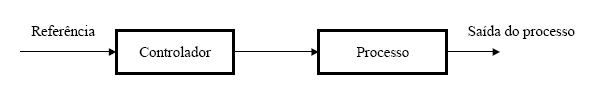
\includegraphics[width=\linewidth]{img/rf-malha_aberta.jpg}
				\caption{Sistema onde utiliza-se Malha Aberta. Sistemas que não possuem realimentação.}
				\label{fig:malha_aberta}
			\end{figure}

			Dessa forma, o processamento de dados é puramente absoluto, sem observar dados de processamento anteriores tendo assim uma visão unicamente momentânea.


		\subsubsection{Malha Fechada}
			Já o sistema de controle em malha fechada, também é denotado de sistema de  controle  por  realimentação.

			A  saída $ y $ é  medida e comparada com   a   saída   desejada,   indicada   através   da referência $ r $,   para processamento  através  do  controlador  e  a  consequente  definição  da  ação  de controle $ u $.

			\begin{figure}[H]
				\centering
				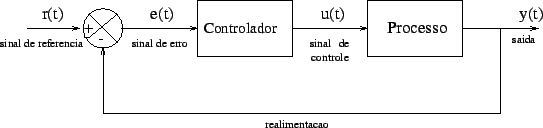
\includegraphics[width=\linewidth]{img/rf-malha_fechada.png}
				\caption{Sistema onde utiliza-se Malha Fechada. Sistemas onde existem um mecanismo de realimentação no controle de determinada ação.}
				\label{fig:malha_fechada}
			\end{figure}

			Neste trabalho é utilizado Malha Fechada. O sistema de realimentação utiliza como entrada, dados de processamentos anteriores criando assim uma proporcionalidade mais autêntica á situação a ser trabalhada.


	\subsection{Sistema Controlador Proporcional Usando Equação Diferencial Lineal de Primeira Ordem} \label{sec:eql1}
		Sistemas de controle é um sistema que possui o propósito de gerenciar o comportamento de outros dispositivos. Pode-se dizer que é uma interconexão de componentes conectados de maneira a comandar, controlar ou ajustar a si mesmo ou outro sistema obtendo uma precisão maior em seus procedimentos.

		A teoria de controladores proporcionais se baseiam em sistemas realimentados. Tais podem ser divididos em basicamente três partes sendo elas:

		\begin{itemize}
			\item Sistema a ser controlado;
			\item Controlador; e
			\item Realimentação.
		\end{itemize}

		O sistema a ser controlado é constituído por atuadores capazes de efetuar as ações necessárias. Os outros dois elementos têm como finalidade fazer com que o desempenho do sistema possua estabilidade e opere com certa precisão e agilidade, seguindo as especificações uma vez estabelecidas. Uma vez estabelecido como o sistema deverá ser desenvolvido, os controladores e sua realimentação serão item essencial para que o processo ocorra de forma estável. Tudo isso pode ser observado no diagrama exibido na Figura \ref{fig:estrutura_sistema_controle}.

		\begin{figure}[H]
			\centering
			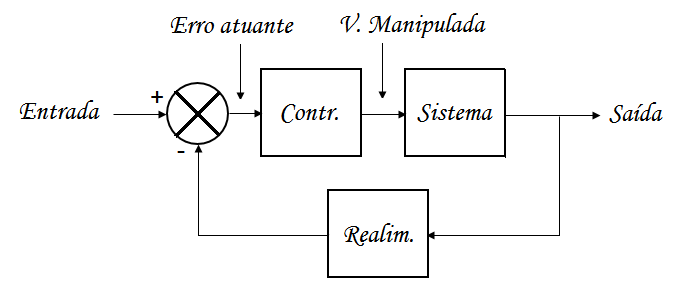
\includegraphics[width=\linewidth]{img/math-realimentacao.png}
			\caption{Estrutura de Sistema de Controle Geral Realimentado.}
			\label{fig:estrutura_sistema_controle}
		\end{figure}

		A realimentação é o ponto chave para a diferenciação de sistemas controladores comuns. Um sistema de controle realimentado compara, instantaneamente, o valor de saída anterior, com o valor de referência existente na entrada do sistema como os sensores. O resultado desta comparação é o centro de toda adaptabilidade estudada e é denominado erro atuante. Este é levado ao controlador, que produz o chamado sinal de controle, cuja função resume-se em reduzir o desvio entre a saída e o sinal desejado. Como o nome sugere, em um controlador proporcional a saída do mesmo, também conhecido como sinal de controle (ou ação de controle), é diretamente proporcional ao sinal de erro, ou seja, ao erro atuante.

		Sabendo-se em da proporcionalidade direta entre o sinal de controle e o sinal de erro, é possível afirmar que

		\begin{equation}
			a(t) \propto e(t)
		\end{equation}

		onde o controle é diretamente proporcional à seu erro.

		Entretanto, não é possível realizar operações matemáticas exatas com o sinal de proporção da fórmula. Par isso, deve-se admitir então uma constante de proporcionalidade entre as mesmas. Esta possui o nome de ganho proporcional e é representado pela variável $f$. Sendo assim

		\begin{equation}
			a(t) = f * e(t) \label{eq:formula_geral}
		\end{equation}

		Dessa forma, o sistema matemático mostrado na Equação \ref{eq:formula_geral} poderá ser representado pelo diagrama exibido na Figura \ref{fig:sistema_dominio_tempo}.

		\begin{figure}[H]
			\centering
			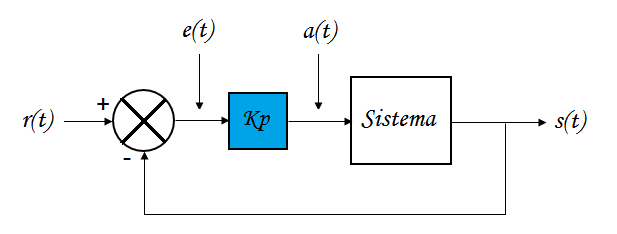
\includegraphics[width=\linewidth]{img/math-diagrama_geral.png}
			\caption{Sistema no Domínio do Tempo Geral.}
			\label{fig:sistema_dominio_tempo}
		\end{figure}

		Sendo assim, como fórmula final, temos

		\begin{equation}
			a(t) = f * (r(t) - s(t))
		\end{equation}

		onde $a(t)$ é a atuação, $e(t)$ representa o erro, $ r(t) $ é o valor de início de execução de controle e $ s(t) $ é saída do controle. Todos representando o valor no tempo $t$.


\section{Elementos do Projeto} \label{sec:elem-teo}

	\subsection{Visão Geral}
		Como já mencionado na Especificação (Seção \ref{sec:especificacao}), existirá dois robores e uma computação em nuvem.

		O trabalho consiste em replicar as ações de um Robô $ \mathcal{A} $ repleto de sensores em um Robô $ \mathcal{B} $ possuindo somente atuadores. Além disso, o processamento de dados e tomada de decisões será totalmente feita em nuvem, deixando os carros unicamente como plataformas de leitura de sensores e atuadores.

		Como é representado na Figura \ref{fig:diagrama}, o Robô $ \mathcal{A} $ terá sensores e atuadores. Seus dados não serão processados nele em si, mas sim em um computador externo ao sistema atuador. Ele fará o trajeto a ele imposto e deverá completá-lo. Após a execução do trajeto, a \textit{cloud} terá dados suficientes, providos de vários sensores, para fazer o Robô $ \mathcal{B} $ realizar o mesmo trajeto sem a utilização de qualquer sensor.

		Para que isso possa ser realizado, cada robô terá seus dispositivos e um componente Wi-Fi para envio e recebimento de dados sem fio à \textit{access points} e assim conexão com a \textit{cloud}.

		\begin{figure}[H]
			\centering
			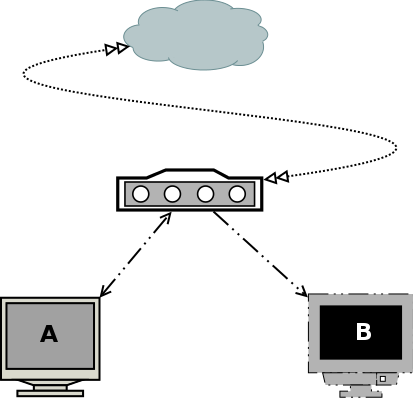
\includegraphics[width=0.5\linewidth]{img/diagrama_geral.png}
			\caption{Diagrama Geral Abstrato do Sistema.}
			\label{fig:diagrama}
		\end{figure}

		Deve-se atentar que os dois robôs possuem características e propósitos diferentes e que todo o processamento é realizado na \textit{cloud} e não nos robôs sendo estes somente para captação de dados e execução de tarefa com seus atuadores.

		Abaixo será descrito cada componente do sistema e algumas propriedades importantes.

	\subsection{Sensores do Robô $ \mathcal{A} $}
		O projeto do Robô $ \mathcal{A} $ terá vários tipos de sensores em várias quantidades diferentes.

		Utilizar somente o sensor fototransistor seria suficiente para o projeto de seguido de linha, mas não para este em si. Este sensor é unicamente para direcionar o carro para que ele não saia da linha completando o trajeto. Usando somente ele, é impossível que o carro saiba sua posição e seus movimentos.

		Para contornar este problema, necessita-se de mais dois tipos de sensores: acelerômetro; e giroscópio. Eles, junto com o fototransistor, serão mencionados nas Seções \ref{sec:fototransistor} e \ref{sec:movimentos}.


		\subsubsection{Sensor de Luz - Fototransistor} \label{sec:fototransistor}

			\paragraph{Tecnologia}
				Para o carro, será utilizado o sensor fototransistor. Em sua superfície, existirá um LED que fará a iluminação da área no qual refletirá sobre a superfície e chegará até o sensor fototransistor. Como o seguidor de linha move sobre dois tipos de superfície (branca e preta), é possível identificar quando ele sairá da direção correta. Essa ideia melhor visualizada com a Figura \ref{fig:ft}.

				\begin{figure}[H]
					\centering
					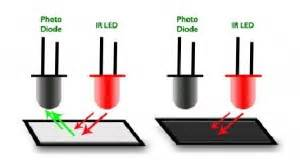
\includegraphics[width=0.45\linewidth]{img/elementos-fototransistor.jpg}
					\caption{Funcionamento do sensor Fototransistor.}
					\label{fig:ft}
				\end{figure}

			\paragraph{Propósito no Projeto}
				O projeto utilizará não somente dois sensores deste tipo mas uma série deles, posicionados logo à extremidade da faixa de direção como é exibido na Figura \ref{fig:dois_sensores}.

				\begin{figure}[H]
					\centering
					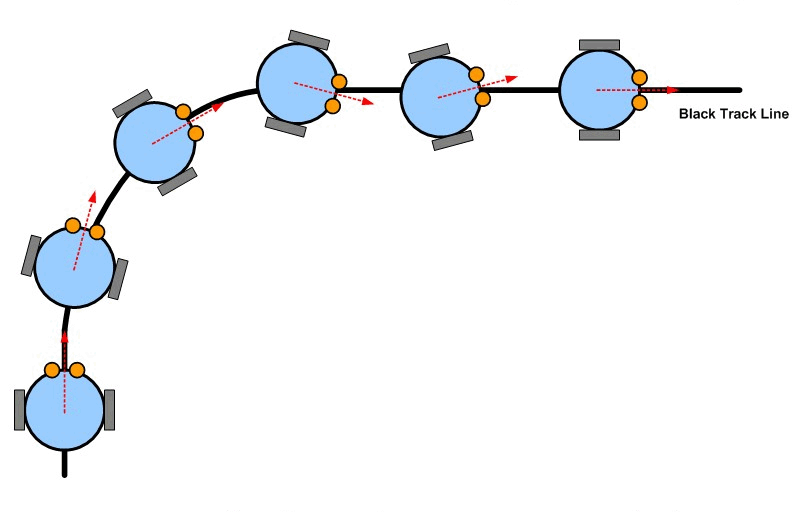
\includegraphics[width=0.9\linewidth]{img/elementos-line_tracking.png}
					\caption{Posição dos Sensores. Exemplo utilizando dois sensores.}
					\label{fig:dois_sensores}
				\end{figure}

				Utilizando uma série de sensores, cada sensor será responsável por avaliar se o carro saiu da linha original. Quanto mais à extremidade a faixa estiver em relação à série de sensores, maior será o erro dela e assim, a consequente uma correção mais rápida. Quanto maior a quantidade de arranjo de sensores melhor será a performance do carro pelo motivo que mais sensores representarão melhor o nível do erro. Por este motivo, será utilizado seis sensores, posicionando três em cada extremidade da faixa. Eles serão dispostos o mais próximo possível de seu adjacente pois a resolução de operação será melhor do que distâncias grandes como três centímetros ou mais. Um exemplo com 8 sensores é exibido na Figura \ref{fig:sensores_series}.

				\begin{figure}[H]
					\centering
					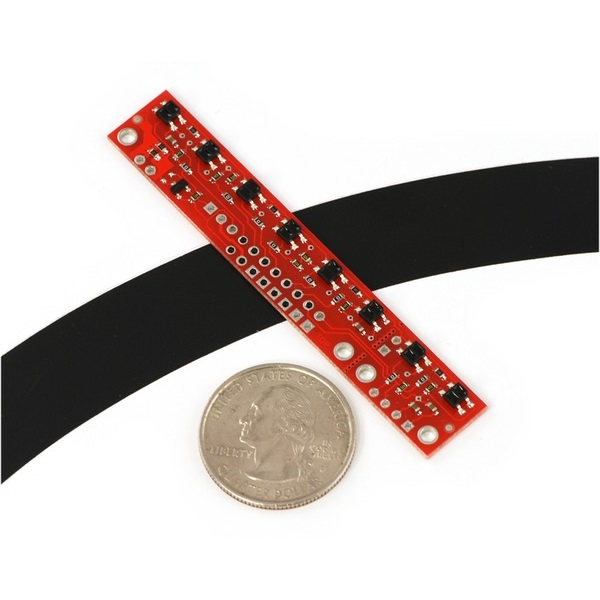
\includegraphics[width=0.7\linewidth]{img/elementos-sensores_series.jpg}
					\caption{Sensores posicionados em uma \textit{board} em série.}
					\label{fig:sensores_series}
				\end{figure}


		\subsubsection{Sensores de Movimento} \label{sec:movimentos}
			Como já descrito \ref{sec:fototransistor}, sensores fototransistores não conseguem realizar gravações de que detectam movimento. Para suprir essa necessidade utilizar-se-á de dois outro tipos de sensores que detectarão movimento. O acelerômetro e o giroscópio.


			\paragraph{Acelerômetro}
				Consegue capturar dados de duas à três dimensões (como mostra a Figura \ref{fig:accelerometer}) podendo reconhecer qualquer tipo de movimento do ambiente onde está instalado.

				\begin{figure}[H]
					\centering
					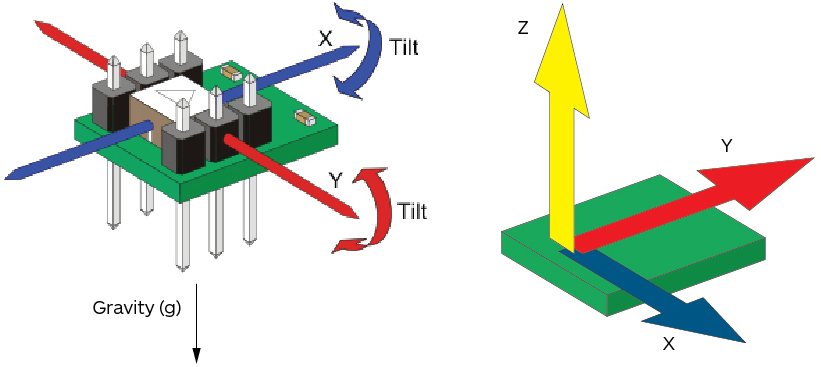
\includegraphics[width=0.9\linewidth]{img/elementos-accelerometer.jpg}
					\caption{Visão técnica sobre o funcionamento do acelerômetro.}
					\label{fig:accelerometer}
				\end{figure}

				O sensor acelerômetro será utilizado para captar dados de deslocamento do carro como aceleração e distância percorrida.

				Entretanto, velocidade e distância também não são suficientes para o projeto do carro como um todo, e por isso será mencionado o uso de giroscópio.


			\paragraph{Giroscópio}
				O giroscópio é um sensor que consegue captar a angulação de determinado objeto à ele instalado, mesmo depois de realizar movimentos.

				Assim, utilizando o aceleração e angulação, é possível registrar o trajeto que o carro realizou ao percorrer a trilha da faixa. Um exemplo da tecnologia utilizada hoje nos dispositivos embarcados é exibido na Figura \ref{fig:gyroscope}.

				\begin{figure}[H]
					\centering
					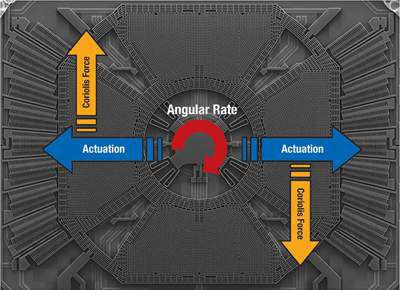
\includegraphics[width=0.6\linewidth]{img/elementos-gyroscope.jpg}
					\caption{Exemplo de giroscópio situado em telefones digitais modernos.}
					\label{fig:gyroscope}
				\end{figure}


			\paragraph{Resultado da Combinação desses Sensores}
				Assim, o sensor fototransistor realizará a leitura do trajeto a ser feito, o acelerômetro receberá a velocidade atual do carro e o giroscópio registrará a angulação do carro.

				Tudo isso processado permite a reprodução exata no Robô $ \mathcal{B} $, mesmo sem utilizar nenhum sensor.


	\subsection{Atuadores}
		O sistema possuirá duas unidades de motores atuadores que serão especificados à seguir.

		\subsubsection{Tecnologia}
			Os motores serão do tipo de Corrente-Contínua, propriedade física que \emph{não} permite o cálculo exato de distância e velocidade do equipamento sem a utilização de sensores de marcação de passo/angulação. Para isso, será utilizado vários sensores para captação de dados do ambiente, onde seus dados serão enviados para a \textit{cloud}, processados e recebidos novamente para assim realizar a atuação no carro. No caso do Carro \textit{B}, não haverá processamento, mas sim a atuação, sendo este somente um receptor escravo.

			Serão acoplados à \textit{board} utilizando um \textit{shield} intermediário entre o microcontrolador e os motores. Tal \textit{shield} realizará o processo de interface de controle e energização dos motores criando assim um sistema estável. Seu nome é L293DD e possui suporte total para interface de pinos NodeMCU. Seu sistema de operação utiliza Ponte-H dupla e com isso é possível controlar até dois motores além de conectores para seleção de interface serial UART, SPI, e entrada analógica, além de conexões para habilitar as opções de \textit{Enable} e \textit{Reset} do microcontrolador. Ele pode ser visto por meio da Figura \ref{fig:eq-motor_shield}.

			\begin{figure}[H]
				\centering
				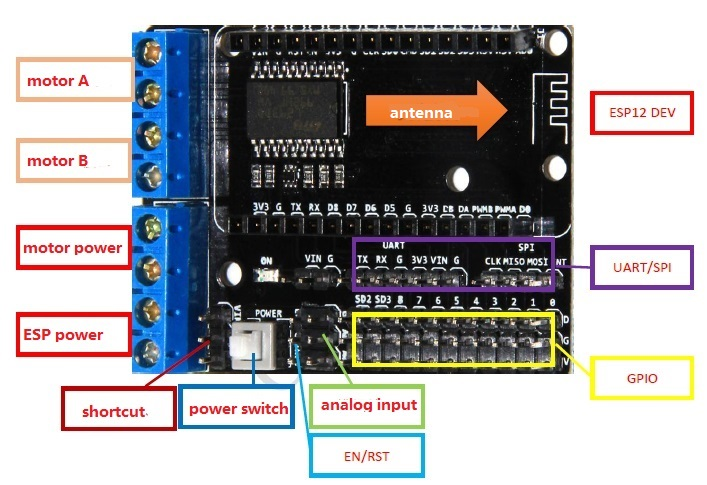
\includegraphics[width=0.9\linewidth]{img/elementos-motor_shield.jpg}
				\caption{Motor \textit{Shield} a ser Utilizado.}
				\label{fig:eq-motor_shield}
			\end{figure}

		\subsubsection{Programação}
			O carro andará numa velocidade máxima fixa em um determinado valor suportado pelos motores. Quando algum de seus sensores, após processados, perceber que o carro saiu da linha, o procedimento de correção de direção será acionada para avaliar os dados dos sensores e assim verificar os passos a serem realizados nos atuadores para que o carro volte a operar normalmente na direção correta em cima da faixa.

			Existem dois tipos de comportamentos em um seguidor de linha comumente conhecido. Eles serão descritos e explicados a seguir.

			\paragraph{Comportamentos Sobre Controle Simples}
				Com controle simples, sem realimentação, é possível perceber que seu erro após à primeiro desvio será grande e sua forma de conserto fará com que ele aumente ainda mais sua margem de erro. isso causará grande distúrbio em seu movimento criando assim um padrão geométrico construído por uma sequência de segmentos lineares alternados quanto à direção, formando linhas quebradas com alternância de ângulos salientes e reentrantes como mostrado na Figura \ref{fig:trajeto2}.

				\begin{figure}[H]
					\centering
					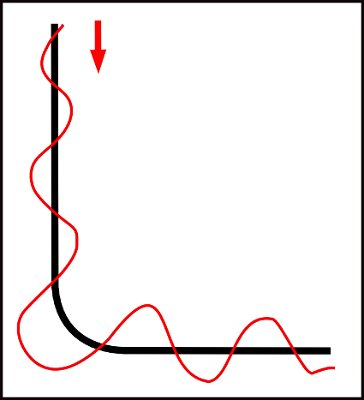
\includegraphics[width=0.5\linewidth]{img/elementos-trajeto2.jpg}
					\caption{Trajeto esperado de um seguidor de linha comum.}
					\label{fig:trajeto2}
				\end{figure}

				Esse movimento oscilatório faz com que o carro gaste tempo em completar sua tarefa de percorrer a linha e também energia, item essencial para sistemas embarcados.

			\paragraph{Comportamentos Sobre Controle Proporcional}
				Utilizando o controle proposto é possível que este padrão seja decrementado ao ponto de tornar o movimento do carro mais suave e portanto seu trajeto mais conciso quanto à linha do trajeto. O resultado esperado é exibido na Figura \ref{fig:trajeto3}.

				\begin{figure}[H]
					\centering
					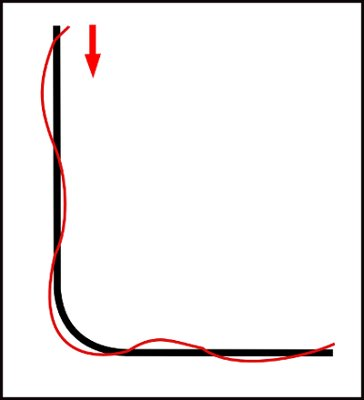
\includegraphics[width=0.5\linewidth]{img/elementos-trajeto3.jpg}
					\caption{Trajeto esperado de um seguidor de linha utilizando Controle Proporcional.}
					\label{fig:trajeto3}
				\end{figure}

				Um fato importante a se atentar é que, para que o carro funcione como esperado, o algoritmo, seus parâmetros e os parâmetros da fórmula de controle proporcional devem estar devidamente calibrados para que o carro obtenha a melhor performance possível.

				Este trajeto faz com que seus movimentos sejam mais suaves, estáveis, ágeis e eficientes em relação ao mostrado na Figura \ref{fig:trajeto2}, exibida anteriormente.


	\subsection{Microcontrolador}
		Microcontrolador utilizado para este trabalho é o NodeMCU. É um plataforma IoT\footnote{\textit{Internet of Things}, ou seja, internet das coisas.} \textit{open-source}.

		Como esperado de um microcontrolador para IoT o sistema possui integrado um componente de comunicação Wi-Fi para troca de dados. Utiliza linguagem de \textit{script} Lua desenvolvida por brasileiros.

		Suas especificações são uma CPU ESP8266 possuindo 128 KB de memória, 4 MB de armazenamento e suporta o sistema operacional chamado XTOS. Permite comunicação pelo Wi-Fi e USB onde também é energizada. Possui um total de 10 pinos de entrada e saída de propósito geral (GPIO) onde suportam funções como PWM, comunicação I$ ^2 $C e 1-wire. Além da antena Wi-Fi, possui também um conversor USB-TTL para comunicação serial.

		Seus microprocessadores podem ser facilmente ligados à um computador e também utilizado a IDE Arduino. A Figura \ref{fig:eq-nodemcu} exibe um esquemático de seu protótipo.

		\begin{figure}[H]
			\centering
			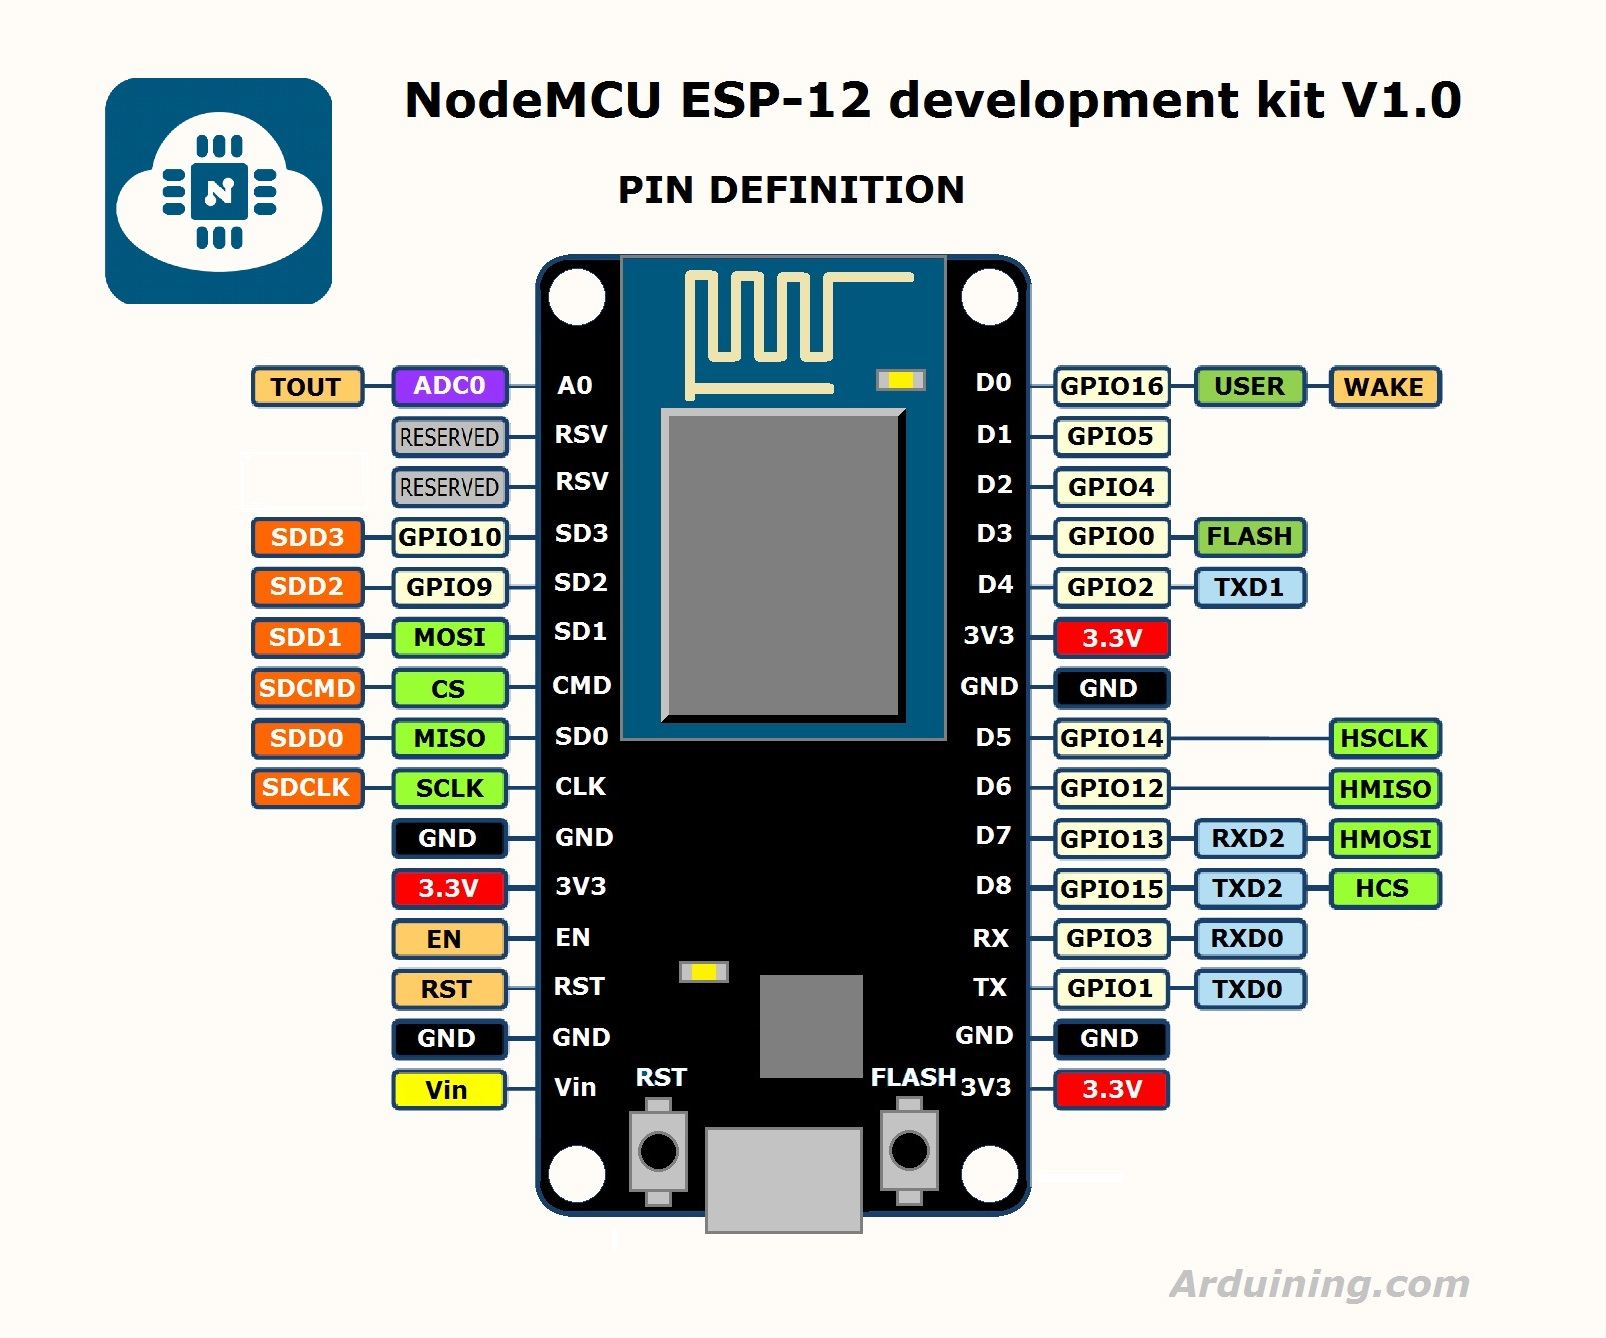
\includegraphics[width=0.96\linewidth]{img/elementos-nodemcu.jpg}
			\caption{O Microcontrolador NodeMCU e seus Componentes e I/O.}
			\label{fig:eq-nodemcu}
		\end{figure}

		Sua programação pode ser feita por diversas maneiras. As duas principais são utilizando um terminal serial para envio de comandos diretamente à placa usando a porta USB do controlador. Para isso, deve-se configurar a comunicação serial para 9600 \textit{baud-rate}. Ao iniciar o controlador, já iniciará informações de comunicação. Feito isso, já é possível enviar comandos ao controlador. Outra forma é utilizando programas para envio de dados até a placa. Eles realizarão toda a `interfaceação' do desenvolvedor com a placa e um exemplo deles é a IDE Arduino.

		Como ela possui placa de comunicação Wi-Fi e um controlador poderoso, é possível também transformá-la num \textit{Web Service} para que realize toda a comunicação sem fio.


	\subsection{Alimentação}
		Sua energização será realizada por meio de fonte externa utilizando pilhas. Isso é necessário pois o sistema completo possui vários componentes que necessitam de uma fonte de energia estável e constante para não afetar no desempenho e também pelo fato do controlador não conseguir fornecer mais que 3.3V e 12mA em suas saídas GPIO.

		Utilizar uma fonte por meio da interface USB diretamente no microcontrolador não seria suficiente para energizar todos os atuadores e sensores do sistema. Dessa forma, a fonte externa alimentará os atuadores e o microcontrolador e este alimentará todos os sensores nele contido.




	\subsection{Nuvem}
		A nuvem será utilizada para processamento, retirando todo o trabalho dos robôs.

		Utilizar este tipo de sistema traz várias vantagens com redução de gasto energia nos robôs e centralização de processamento e \textit{backup} de informações em local seguro além da transparência do sistema de controle.

		Entretanto, latências altas em comunicações ou pacotes de informações corrompidas podem tornar o sistema inconsistente ou até mesmo comprometido.

		A arquitetura do sistema será melhor detalhada em Arquitetura de Comunicação, Seção \ref{sec:arch}.


\section{Modelamento Matemático} \label{sec:math}

	\subsection{Teoria da Equação Diferencial Linear}
		Equações Diferenciais Lineares são equações que suas soluções podem ser somadas a fim de produzir uma nova solução.

		É considerada linear quando satisfaz as características de que cada coeficiente a $a_{n}$ e o termo de não-homogeneidade só dependem da variável independente, no caso $x$; e a variável dependente, no caso $y$, e suas derivadas são de primeiro grau. Assim, ela deve representar a seguinte forma

		\begin{equation}
		f(x) = a_{n}(x)\frac{d^{n}y}{dx^{n}} + a_{n-1}(x)\frac{d^{n-1}y}{dx^{n-1}} + \cdots +  a_{1}(x)\frac{dy}{dx} + a_0(x)y
		\end{equation}

		\begin{comment}
			No uso para problemas que utilizam Controle Proporcional descrito no Seção \ref{sec:controle_proporcional}, basta desligar todas as derivadas e integrais da equação obtendo \todo{Deixa isso?}

			\begin{equation}
			f(x) = a_{n}(x) + a_{n-1}(x) + \cdots +  a_{1}(x) + a_0(x)y
			\end{equation}
		\end{comment}


	\subsection{Definições}
		%https://syclops.wordpress.com/2011/08/06/part-2-line-following-robot-code-guideline-arduino-using-pid/
		Para iniciar a discussão sobre sistema de controle proporcional, primeiramente será definido os termos utilizados.

		\begin{description}
			\item[\textit{Alvo:}] É a posição que desejamos que o carro esteja em relação à faixa, ou seja, centralizado respeitando a devida linha.

			\item[\textit{Erro:}] Diferença entre a posição atual e o \textit{Alvo}. Pode ser qualquer valor no conjunto dos ${\rm I\!R}$.

			\item[\textit{Proporção:}] Fator que determinará quão distante o carro está da linha. Por exemplo são as proporções: `\textit{para a esquerda}',  `\textit{para a direita}', `\textit{para a extrema esquerda}', `\textit{pouco para a direita}', etc. É representado pela constante de variação $ K_p $.

			\begin{comment}

			\item[\textit{Integral:}] Proporciona o erro acumulado sobre o tempo corrido. Isso significa que este irá informar se o carro vem estando na linha nos últimos momentos ou não. Representada pela constante de variação $ K_i $.

			\item[\textit{Derivada:}] Taxa no qual exibe a oscilação do robô sobre a linha, representada pela constante de variação $ K_d $.
			\end{comment}

		\end{description}

		%Ambos \textit{Integral} e \textit{Derivada} utilizam o valor \textit{Proporção}.

		O procedimento de execução é baseado no seguinte pseudocódigo:
		\begin{enumerate} \it
			\item Realiza o cálculo inicial da posição atual.

			\item Calcula o erro baseado na posição atual.

			\item Ele então comandará os motores para fazer uma girada:
			\begin{itemize}
				\item \underline{Brusca} caso o erro for grande; ou
				\item \underline{Leve} caso o erro for pequeno.
			\end{itemize}
			Assim, basicamente, a magnitude do giro tomado é proporcional ao \textit{erro}.

			\item Repete os passos até completar o objetivo inicial.
		\end{enumerate}

		Com esses passos, saímos de um controle simples para um Contro Proporcional mais eficaz.

		\begin{comment}


		Mesmo se depois desses passos o valor de \textit{erro} não decrementar ou decrementar de forma bem lenta, ao realizar o passo 4, o controlador fará uma nova avaliação incrementando a magnitude de conserto de posição realizando novamente de forma mais brusca a tentativa de posicionar o carro novamente à posição centralizada. Esse processo só é possível por causa do Controle Integral. O efeito de redução de oscilação por tempo é trabalho pelo Controle Derivativo.

		O Controlador Proporcional Integral-Derivativo, também chamado de Controlador PID, é uma metodologia de cálculo de controle de processo que une várias outras menores. Utiliza de teorias como as Ações Derivativa (Controle PD), Integral (Controle PI) e Proporcional (Controle P).

		Estes quatro modos de controle, incluindo PID, são também designados de ações de controle, cada uma delas reagindo de forma distinta ao erro presente nos sistemas. O controle:

		\begin{itemize}
			\item Proporcional: ajusta a variável de controle de forma proporcional ao erro;
			\item Integral: ajusta a variável de controle baseando-se no tempo em que o erro acontece;
			\item Derivativo: ajusta a variável de controle tendo como base a taxa de variação do erro; e
			\item A combinação destes tipos de controle forma o controlador PID.
		\end{itemize}

		\end{comment}

		São amplamente utilizados em situações que se baseiam em controladores eletrônicos chamados ``\textit{single-loop}''.

		Abaixo é descrito a formulação matemática do conceito de controlador proporcional

		%Como ele é formado por todos os outros controles, será descrito brevemente cada um deles.


	\subsubsection{Teoria de Controle Proporcional (P)} \label{sec:P}
		Produz um sinal de saída que é proporcional à parâmetro do erro

		\begin{equation}
		P_{\mathrm {saida} }=K_{p}\,{e(t)}
		\end{equation}

		onde:

		\begin{description}
			\item[$ e(t) $\textit{:}] Erro no tempo $ t $.
			\item[$ K_p $\textit{:}] Constante relativa à proporção.
		\end{description}

		Esse método possui a propriedade de eliminar as oscilações do sinal de saída. Para tal, o sistema permanece sempre ligado e o sinal de saída é diferente de zero.


	\subsection{Funcionamento Teórico-Procedural}
		Aqui será descrito uma representação de como será a implementação de toda a teoria descrita neste trabalho. Assim, de forma geral, teremos o seguinte algoritmo implementado para tratamento dos valores obtidos dos sensores e ajuste da rotações dos motores.

		\begin{algorithm}[H]
			\caption{Controle Proporcional de Correção de Angulação}\label{euclid}
			\begin{algorithmic}[1]
				%\Procedure{proportional\_control}{$ position, set\_point, \Delta, \int, last\_\Delta, y', \Phi $}
				\Procedure{proportional\_control}{$ position, set\_point, \Delta, last\_\Delta, \Phi $}

				\State $ \Delta \gets position - set\_point $
				%\State $ \int \gets \int + \Delta $
				%\State $ y' \gets \Delta - last\_\Delta $
				\State $ \Phi \gets \Delta * K_p $
				%\State $ \Phi \gets \Delta * K_p + \int * K_i + y' * K_d $
				\EndProcedure
			\end{algorithmic}
		\end{algorithm}

		onde:

		\begin{description}
			\item[\textit{position:}] Posição atual do carro.

			\item[\textit{set\_point:}] Ponto central onde encontra-se a faixa.

			\item[$ \Delta $\textit{:}] Representa o erro proporcional da posição atual contra o ponto central da faixa.

			%\item[$ \int $\textit{:}] Representa o acúmulo de erro atual.

			\item[$ last\_\Delta $\textit{:}] Representa o erro proporcional da posição da iteração passada.

			%\item[$ y' $\textit{:}] Retêm a diferença entre os erros atual e da iteração anterior.

			\item[$ \Phi $\textit{:}] Correção a ser realizada nesta iteração.
		\end{description}

		Como é de se esperar, a correção proporcional $ \Phi $ será aplicada à velocidade motor para conserto de posição do carro.


\section{Arquitetura de Comunicação} \label{sec:arch}

	%http://bbs.smartarduino.com/showthread.php?tid=3
	%http://bbs.smartarduino.com/showthread.php?tid=2
	\subsection{\textit{Clouds} Disponíveis}
		Nesta seção, será relatado onze serviços de \textit{cloud computing} que podem ser acessados gratuitamente com recursos limitados para teste e avaliação.

		\begin{itemize}
			\item Microsoft Azure; % precisa de cnpj
			\item Amazon Web Services (AWS);
			\item IBM Bluemix;
			\item BMC Software;
			\item Computer Associates;
			\item Cisco Systems;
			\item Hewlett-Packard Cloud Computer;
			\item Intel Cloud Computer;
			\item Doit Cloud;
			\item Oracle Cloud Computer; e
			\item Google Cloud Plataform.
		\end{itemize}

		Abaixo é descrito algumas informações e propriedades de alguns serviços prestados.

		\subsubsection{Amazon \textit{Web Services} (AWS)}
			O serviço fornecido pela Amazon possui várias vantagens e facilidades de uso. Um adentro ao tema, o Amazon \textit{Web Services} (AWS) é um subconjunto de operações de computação na nuvem da \href{https://www.amazon.com}{\textit{amazon.com}}.

			Ela oferece recursos \textit{on-demand} onde opera em mais de 16 regiões geográficas pelo mundo e uma delas encontra-se em São Paulo, no Brasil. Neste pacote, também é incluso o Amazon \textit{Elastic Compute Cloud} e também o Amazon \textit{Simple Storage Service} como ferramentas adicionais para uso.

			Ao final de 2016, AWS já possuía mais de 70 serviços na nuvem incluindo serviços próprios para IoT. Entretanto, o sistema deve executar sistemas operacionais ou linguagens de programação \textit{Node.js}, \textit{Java} ou \textit{Python} sendo esses requisitos não adaptáveis ao dispositivos obtidos no momento.

		%\subsubsection{Google Cloud Plataform}


		\subsubsection{Oracle Cloud Computer}
			Necessita compra pra uso do sistema de controle IoT dos serviços prestados. Outra desvantagem de uso acadêmico é que seus serviços são cobrados assim que o prazo de teste acaba sem solicitação prévia.


		\subsubsection{Google Cloud Plataform}

			Empresas como Coca-Cola, Spotify, Philips, utilizam este serviço para processamento massivo de dados e terceirização de serviços de infraestrutura de projeto como redundância, técnicas de \textit{failover}, backups, monitoramento e armazenamento de grandes volumes de dados.

		\begin{comment}

		\subsubsection{Microsoft Azure}
		É um serviço de computação na nuvem criada pela Microsoft para construção, desenvolvimento e gestão de aplicações e serviços por meio de uma rede global de \textit{data centers} da própria empresa.

		Tem suporta à várias linguagens de programações diferentes além de um total de mais de 600 serviços disponíveis para uso.


		\subsubsection{Amazon \textit{Web Services} (AWS)}
		Amazon \textit{Web Services} (AWS) é um subconjunto de operações de computação na nuvem da Amazon.com.

		Ela oferece recursos \textit{on-demand} onde opera em mais de 16 regiões geográficas pelo mundo e uma delas encontra-se em São Paulo, no Brasil. Neste pacote, também é incluso o Amazon \textit{Elastic Compute Cloud} e também o Amazon \textit{Simple Storage Service} como ferramentas adicionais para uso.

		Ao final de 2016, AWS já possuia mai de 70 serviços na nuvem incluindo IoT.

		\subsubsection{IBM Bluemix}

		\subsubsection{BMC Software}

		\subsubsection{Computer Associates}
		Possui uma extensa coleção de computação em nuvem e \textit{software} de pesquisas empresariais

		\subsubsection{Cisco Systems}

		\subsubsection{Hewlett-Packard}

		\subsubsection{Intel}

		\subsubsection{Oracle}

		\subsubsection{Google Cloud Plataform}

		Empresas como Coca-Cola, Spotify, Philips, utilizam este serviço para processamento massivo de dados e terceirização de serviços de infraestrutura de projeto como redundância, técnicas de \textit{failover}, backups, monitoramento e armazenamento de grandes volumes de dados.
		\end{comment}


	\subsection{Arquitetura}
		\subsubsection{Descrição Geral de Operação}

		Será estabelecida uma comunicação TCP entre todos os dispositivos, propriedade que utiliza \textit{hand-shake} e verificação de perda de pacotes.

		Uma vez a comunicação esteja estabelecida, a \textit{cloud} receberá um comando de início de envio de dados, os dados propriamente ditos e a finalização do envio. Novamente, ao utilizar o protocolo TCP, não é necessário realizar verificação de recebimento e também de \textit{ack}. Como o Robô $ \mathcal{A} $ não realiza processamento, os dados recebidos pela \textit{cloud} serão processados para retorno ao Robô $ \mathcal{A} $ e assim sua atuação.

		Além de processar na \textit{cloud}, as informações coletadas e processadas serão utilizadas para conduzir os atuadores do no Robô $ \mathcal{B} $, repetindo os passos realizados pelo primeiro, sem a utilização de qualquer sensor para auxiliar na obtenção de seu propósito. Deve-se lembrar que toda a explicação descrita no Referencial Teório (Seção \ref{sec:rt}) e a fundamentação matemática descrita neste trabalho na Seção \ref{sec:math} serão de fato implementadas na \textit{cloud}.

		Dessa forma, a \textit{cloud} terá dois papeis principais neste sistema como um todo, sendo eles:

		\begin{enumerate}
			\item Realizar \textit{todo} o processamento do \textit{Line Tracker} do Robô $ \mathcal{A} $;
			\item Armazenar, computar e enviar os dados obtidos do Robô $ \mathcal{A} $ para o Robô $ \mathcal{B} $ a fim de que ele consiga executar a mesma tarefa  de A, inúmeras vezes se necessário, sem utilização de qualquer equipamento auxiliar.
		\end{enumerate}


	\subsection{Protocolarização}

		\subsubsection{Temporização}
			Será definido dentro do Robô $ \mathcal{A} $ um intervalo fixo $ t $ para captação e envio de dados à \textit{cloud}.

			Criando um padrão igual este, é possível reproduzi-lo no Robô $ \mathcal{B} $, com uma precisão maior de reprodução de movimentos capturados pelo Robô $ \mathcal{A} $. Ao final, poderá ser enviado ao Robô $ \mathcal{B} $ os dados nos devidos tempos corretos de execução, ou mesmo um vetor com todos os dados nos devidos tempos corretos já preparados para a execução.


%\section{Códigos}
	\subsection{Código em Linguagem Arduino}
	\begin{minted}
		[
		frame=lines,
		framesep=2mm,
		tabsize=3,
		breaklines=true,
		baselinestretch=1.2,
		fontsize=\scriptsize,
		linenos
		]{C}
		
		// Cálculos usados para calcular média
		long media_sensores;
		int somatorio_sensores;
		
		// Posicao do veículo
		int posicao;
		
		int quant_sensores = 6;
		long sensores[]    = {0, 0, 0, 0, 0, 0};
		
		void setup(){
			Serial.begin(9600);
		}
		
		void loop(){
			leitura_sensores();                      // Reads sensor values and computes sensor sum and weighted average
			calculo_proporcao();                     //Calculates posicao[set point] and computes Kp,Ki and Kd
			calculo_giro();                          //Computes the error to be corrected
			atuacao_motor(velocidade_direito, velocidade_esquerdo);  //Sends PWM signals to the motors
		}
	
		void leitura_sensores() {
			media_sensores     = 0;
			somatorio_sensores = 0;
			for (int i = 0; i < quant_sensores; i++){
				sensores[i] = analogRead(i);
				
				media_sensores += sensores[i] * i * 1000;     //Calculating the weighted mean of the sensor readings.
				somatorio_sensores += int(sensores[i]);       //Calculating sum of sensor readings.
				
			}
		}
	
		void calculo_proporcao(){
			posicao   = int(media_sensores / somatorio_sensores);
			proporcao = posicao – posicao_perfeita;      // Replace posicao_perfeita by your set point
			integral  = integral + proporcao;
			derivada  = proporcao - ultima_proporcao;
			ultima_proporcao = proporcao;
			
			valor_erro = int(proporcao * Kp + integral * Ki + derivada * Kd);
		}
	
		
		void calculo_giro(){  //Restricting the error value between +256.
			if (valor_erro< -256){ valor_erro = -256;     } if (valor_erro> 256){
				valor_erro = 256;
			}
			
			// If valor_erro is less than zero calculate right turn speed values
			if (valor_erro< 0){
				velocidade_direito  = velocidade_maxima + valor_erro;
				velocidade_esquerdo = velocidade_maxima;
			}
			
			// Ifvalor_erro is greater than zero calculate left turn values
			
			else{
				velocidade_direito  = velocidade_maxima;
				velocidade_esquerdo = velocidade_maxima - valor_erro;
			}
		}
	
	
		void atuacao_motor(intvelocidade_direito, intvelocidade_esquerdo){
			// Drive motors according to the calculated values for a turn
			analogWrite(motor_direito, velocidade_direito);
			analogWrite(motor_esquerdo, velocidade_esquerdo);
			delay(60);
		}
		
	\end{minted}

\end{document}
